\chapter{Einführung in den Versuch}
\label{cha:einfuehrung}
\todo{}
\section{Einleitung}

Die Im Rahmen dieses Projekts zu behandelnde Aufgabe ist der Aufbau eines Netzwerks aus Sensoren.
Während des HT2024 und des WT2025 hat sich unsere Gruppe mindestens einmal wöchentlich getroffen.
Das Projekt umfasste sowohl die Planung, als auch die Durchführung und Auswertung von Messaufbauten und Versuchen.
Als Grundlage diente ein bereits bestehender Versuchsaufbau an einem Fahrrad, siehe \ref{cha:alteraufbau}.
Da im Laufe des Projekts in verschiedenen Entwicklungsteams gearbeitet wurde und jede Gruppe eigenständig an ihren Berichten arbeitete kann es zu Doppelungen im Bericht kommen.

\section{Zielsetzung}
Ziel des Projekts ist es den bestehenden Aufbau am Fahrrad weiterzuentwickeln und zu verbessern.
Dies soll durch die Verwendung des VLINK200 Nodes der Herstellers LORD/HBK stattfinden.
Dieses Unternehmen bietet Lösungen für drahtlose Sensornetzwerke an. Diese werden in der Industrie und dem Internet of Things, sowie auch in der Forschung und im Maschinen und Anlagenbau verwendet.
Dort wird sie vor allem im Bereich der predictive Maintenance eingesetzt.
Der Node verfügt über 8 Eingänge, 4 ±156mV Differenzeingänge und 4 ± 156mV Single-Ended Eingänge.
Er gewährleistet eine verlustfreie Datenübertragung sowie auch die Speicherung von Messdaten.
Man kann den Node über interne, austauschbare Batterien und externe Akkus betreiben.

\begin{figure}[h]
    \begin{center}
        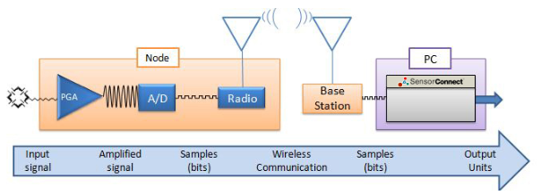
\includegraphics[width=1\textwidth, keepaspectratio]{lord_wireless.png}
        \caption[LORD drahtlose Übertragung (Abbildungsverzeichnis)]{LORD drahtlose Übertragung
        \cite{VLInkManual}
        }
        \label{fig:lordwireless}
    \end{center}
\end{figure}

Abbildung \ref{fig:lordwireless} zeigt die Funktionsweise der drahtlosen Datenübertragung.
Ein an das Node angeschlossener Sensor wird inerhalb des Nodes verstärkt und digitalisiert.
Anschließend werden die Messdaten vom Node drahtlos an eine Base Station gesendet welche mit einem Laptop verbunden ist.
Dort kann durch die Software SensorConnect auf den Node zugegriffen werden und dessen Daten visualisiert oder weiter verarbeitet werden.


Abbildung \ref{fig:lordproducts} zeigt einen Teil der Produktpalette.
Als Gateway wurde von uns der dort gezeigte USB Stick genutzt.
Insgesamt wurden uns zwei VLINK 200 Node, und ein USB Stick zur Verfügung gestellt was in der späten Projektphase teilweise zu Problemen führte,
siehe \ref{sec:probleme} \nameref{sec:probleme}.

\begin{figure}[h]
    \begin{center}
        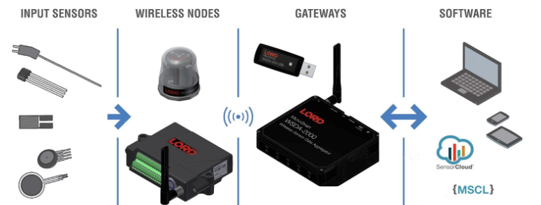
\includegraphics[width=1\textwidth, keepaspectratio]{lord_products.png}
        \caption[LORD Produkte (Abbildungsverzeichnis)]{LORD Produkte
        \cite{VLInkManual}
        }
        \label{fig:lordproducts}
    \end{center}
\end{figure}

\section{Aufgabenverteilung}
Aufgrund der Gruppenstärke von fünf Studenten erschien es sinnvoll zunächst eine Aufgabenverteilung und Aufteilung in Teams durchzuführen.
Nachdem sich jeder mit der Aufgabenstellung und den notwendigen theoretischen Grundlagen vertraut gemacht hatte geschah die Aufteilung in die Teams Fahrrad (Bellgardt, Menzel) und Flying Suit (Grote, Nerb, Ulit).
Zu einem späteren Zeitpunkt hat sich vom Team Flying Suit das Team Software (Grote) abgespaltet, siehe Abbildung \ref{fig:aufgabenverteilung}.

\begin{figure}[h]
    \begin{center}
        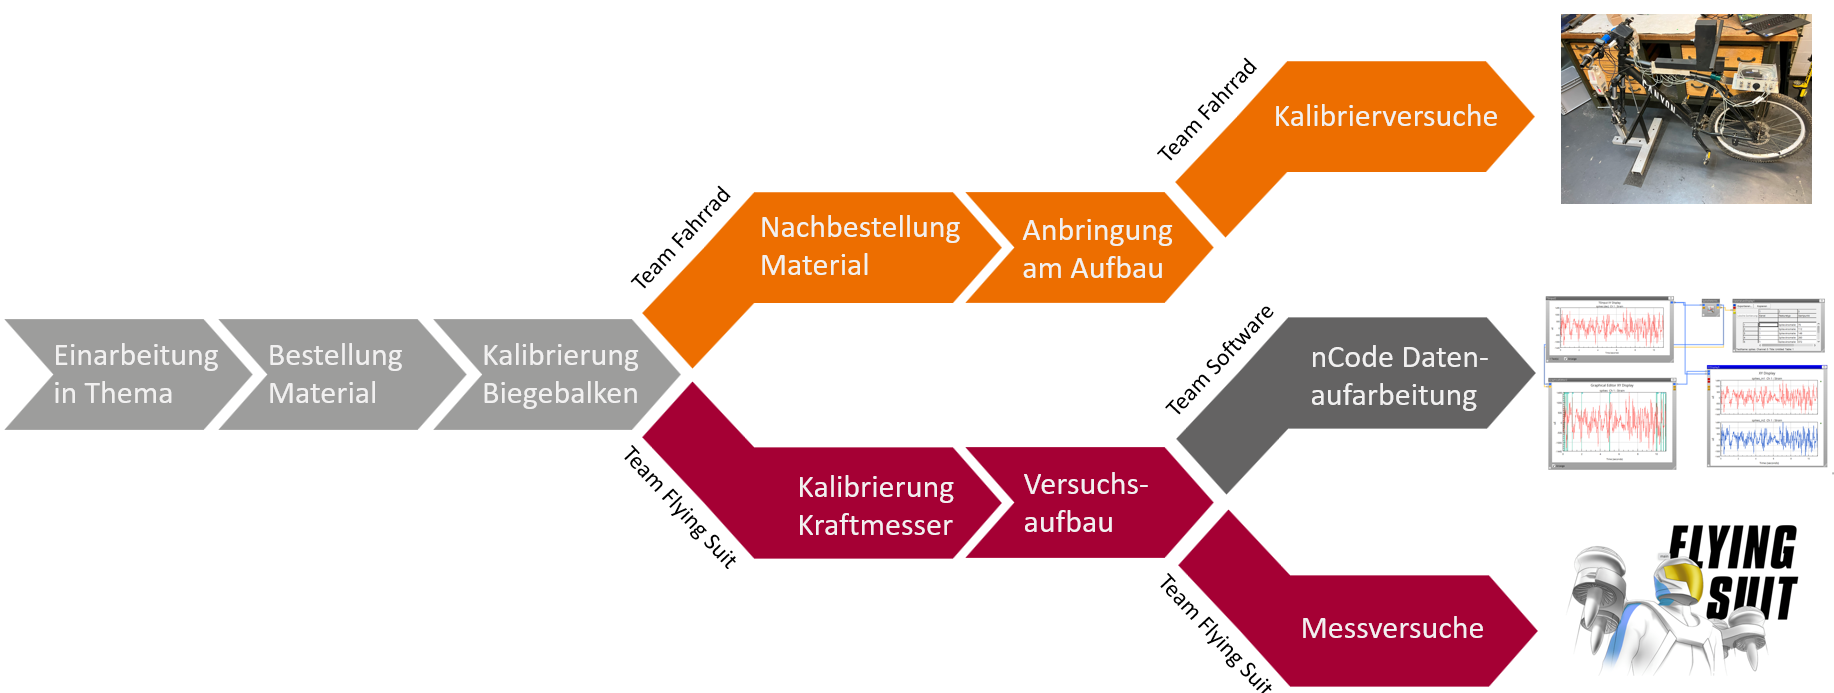
\includegraphics[width=1\textwidth, keepaspectratio]{aufgabenverteilung.png}
        \caption[Aufgabenverteilung Entwicklungsteams (Abbildungsverzeichnis)]{Aufgabenverteilung Entwicklungsteams
        %\cite{VLInkManual}
        }
        \label{fig:aufgabenverteilung}
    \end{center}
\end{figure}